\chapter{SikuliX}
	\section{Instalace}
	Po stažení balíčku započne instalace jeho spuštěním\footnote{Je potřeba instalace JRE nebo JDK 6 a~vyšší, v~linuxové distribuci balíky \emph{libopencv-core2.4, libopencv-imgproc2.4, libopencv-highgui2.4, libtesseract3} a~\emph{wmctrl} \citep{SikuliX}}. Je ukázána instalace v~Linuxu, avšak instalace ve Windows je obdobná. V~průběhu máme na výběr různé možnosti, jak chceme nástroj používat, viz obrázek \ref{Instal}. Např. zda chceme používat SikuliX-IDE a~Python nebo Ruby, jestli budeme používat jiné IDE a~Javu a~zda chceme používat OCR funkce. Zaškrtneme všechna políčka kromě \emph{Ruby (JRuby)} a~klikneme na \emph{Setup Now}. Jsme dotázáni, zda chceme balíčky stáhnout, nebo ukončit instalaci. Zvolíme \emph{Yes}. Další dotaz je na verzi Jythonu, kterou chceme použít, s~upozorněním, že může nastat problém se znaky v~kódování UTF-8. Opět zvolíme \emph{Yes}. Začne vytváření souborů a~měla by se otevřít dvě okna jako na obrázu \ref{InstalOK}, obě potvrdíme tlačítkem \emph{OK}. Pokud vše proběhne v~pořádku, vzniknou v~adresáři soubory podobné těmto\footnote{Může se lišit na různých OS} \emph{runsikulix, SetupStuff, SikuliX-1.1.0-SetupLog.txt, sikulixapi.jar, sikulix.jar}.
	\begin{figure}[ht!]
		\centering
		\caption{Instalace SikuliX}
		\label{Instal}
		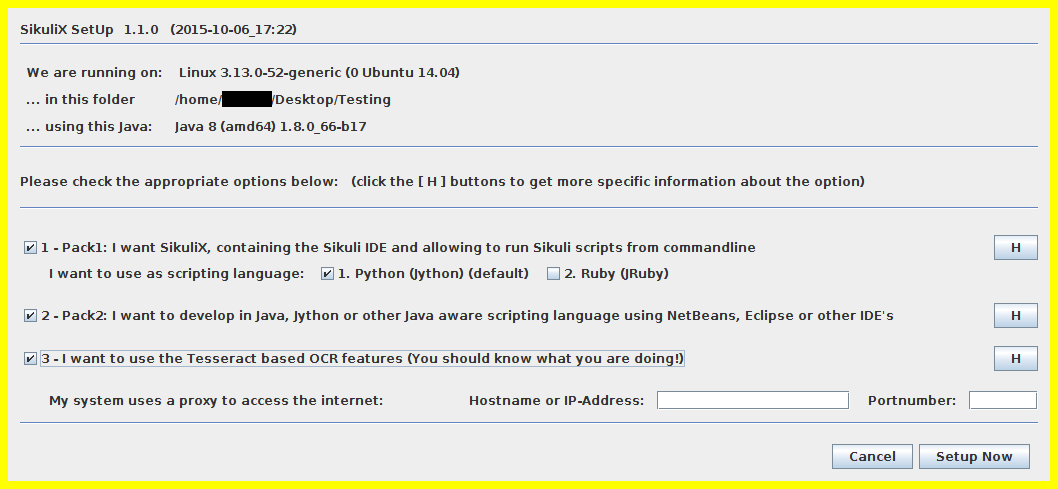
\includegraphics[width=13.5cm]{img/Instalace/Instalace.png}
	\end{figure}
	\begin{figure}[ht!]
		\centering
		\caption{Test instalace}
		\label{InstalOK}
		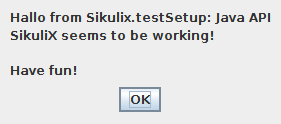
\includegraphics[width=9cm]{img/Instalace/InstalaceOK.png}\\[0.3cm]
		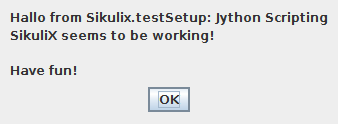
\includegraphics[width=9cm]{img/Instalace/InstalaceOK1.png}
	\end{figure}
	
	\section{Tvorba testů}
	Pro tvorbu testů pomocí SikuliX jsou nejdůležitější snímky (screenshoty) řídících prvků, které bude SikuliX hledat a~případně používat k~některým akcím. Je tedy vhodné si nejprve aplikaci spustit, vybrat příslušné prvky a~vytvořit jejich snímky. Při jejich tvorbě se doporučuje preciznost a~přesnost, neboť v~jistých situacích mohou nastat problémy, které budou zmíněny později.
	
	Pokud je snímků více, je vhodné je třídit do adresářů. To není nutné, ale zlepšuje to čitelnost kódu a~usnadňuje práci s~nástrojem. Adresáře mohou např. sdružovat snímky prvků, které jsou si nějakým způsobem podobné (tlačítka, textová pole, výběrové seznamy, chybové hlášky, apod.). Stejně tak je vhodné snímky pojmenovávat na základě toho, co obsahují (vstupní textové pole, label Vstup, apod.).
	
	Dle \citep{SikuliXImgs} SikuliX interně používá třídu ImageIO z~Javy. Podporované formáty jsou tedy bmp, wbmp, jpg, jpeg, png a gif. Vzhledem k~vlastnostem se doporučuje používat formát png.
	
	Pokud je vytvářený test jednoduchý a~není potřeba většího množství testů, je jednodušší vytvořit jej pomocí SikuliX-IDE. Pokud však chceme aplikaci testovat podrobněji a~psát velké množství testovacích případů, je vhodnější použít některý z~podporovaných programovacích jazyků a~využít tak jeho možnosti jako nadstavbu nad SikuliX.
	
	\section{SikuliX-IDE}
	Dle \citep{SikuliX} je možné SikuliX-IDE spustit různými způsoby:
	\begin{enumerate}
		\item Spuštěním souboru SikuliX.app (Mac) nebo SikuliX.exe (Windows),
		\item dvojklikem na soubor runsikulix (Linux) nebo runsikulix.cmd (Windows),
		\item z~příkazové řádky příkazem\\
		\texttt{java -jar cesta/k/sikulix.jar [volitelne parametry]}
	\end{enumerate}
	Po spuštění vypadá IDE jako na obrázku \ref{SikuliXIDE}. Jako parametry se v~metodách, ve kterých je to možné, ukazují obrázky vzorů, podle kterých se na obrazovce nástroj orientuje, případně cesta k~nim.
	\begin{figure}[ht!]
		\centering
		\caption{SikuliX-IDE}
		\label{SikuliXIDE}
		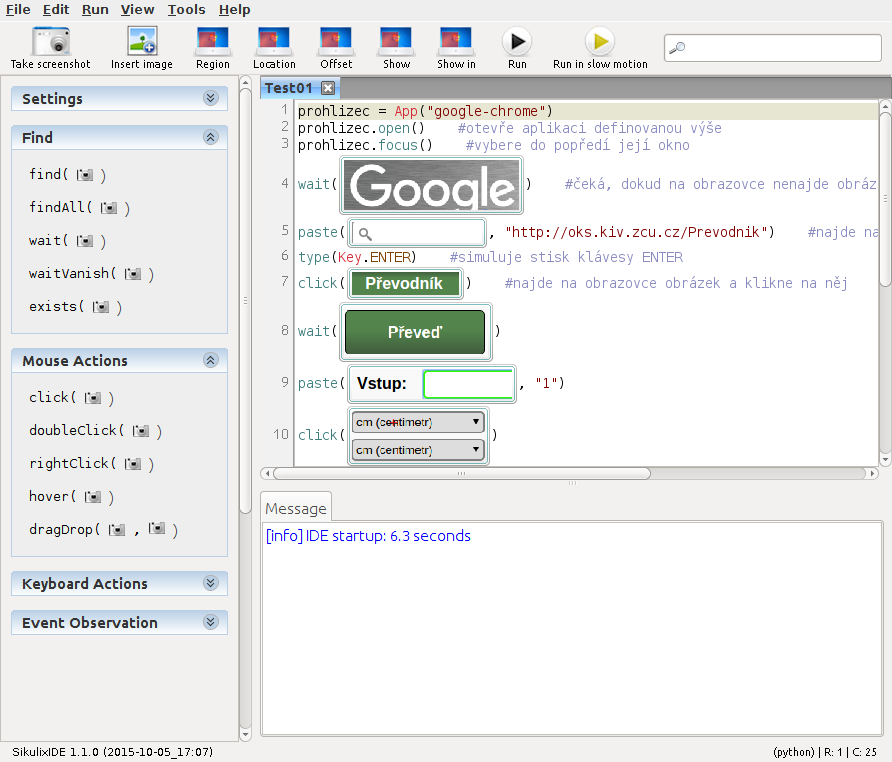
\includegraphics[width=13.5cm]{img/SikuliXIDE.png}
	\end{figure}
	
		\subsection{První skript}
		Skript se připravuje v~SikuliX-IDE, které je vidět na obrázku \ref{SikuliXIDE}. Kód, který je vidět v~\ref{PrvniSkript}, nemusí být v~IDE identický, ale cesta k~obrázku může být nahrazena jeho náhledem, pokud je tato možnost zvolena v~nastavení nástroje. K~tvorbě jsou v~IDE užitečné pomůcky, které se nacházejí v~levém a~v~horním panelu.
		
		Pro spuštění aplikace (např. webového prohlížeče) se do příslušné metody zadá cesta k~jeho spustitelnému souboru. Pokud se používá OS Linux, stačí zadat terminálový příkaz pro spuštění (např. \texttt{"google-chrome"}, \texttt{"firefox"}, apod.).
		
		Skript pracuje tak, že se otevře prohlížeč, který přejde na adresu \url{http://oks.kiv.zcu.cz/Prevodnik}. Klikne na odkaz \emph{Převodník}, do vstupního pole vloží \emph{1} a~stiskne \emph{Převeď}. Z~pole s~výsledkem přečte text a~porovná jej s~předpokládanou hodnotou \emph{2,54}. Pokud si odpovídají, objeví se dialogové okno s~potvrzením, jestliže ne, zobrazí se chybová hláška. Obdobně je tomu v~následující části, kde se pouze kontroluje existence obrázku.
		\\[\topsep]Pro vytvoření skriptu postupujeme následovně:
		\vspace{-\topsep}
			\begin{enumerate}
				\item Spustíme SikuliX-IDE jednou z~výše uvedených metod.
				\item Napíšeme kód pro otevření a~vybrání okna prohlížeče do popředí:\\\texttt{prohlizec = App("google-chrome")\\prohlizec.open()\\prohlizec.focus()}
				\item Spustíme prohlížeč.
				\item V~SikulixIDE v~levém menu klikneme na 
\includegraphics[scale=0.7]{img/PrvniSkript/wait.png} a~provedeme screenshot statické části aplikace. Skript tedy bude vypadat přibližně takto:
					\begin{figure}[ht!]
						\centering
						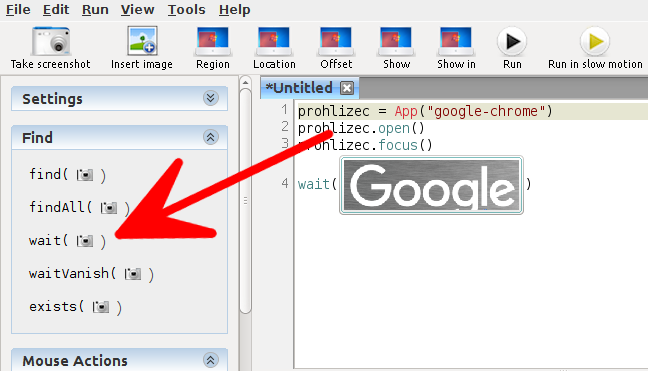
\includegraphics[width=12.5cm]{img/PrvniSkript/krok4.png}
					\end{figure}
					\FloatBarrier
				\item V~levém menu otevřeme podmenu \emph{Keyboard Actions} a~vybereme\\
\includegraphics[scale=0.7]{img/PrvniSkript/paste.png}. Nyní provedeme screenshot políčka pro URL adresu a~jako druhý parametr funkce zadáme URL adresu aplikace Převodník (\url{"http://oks.kiv.zcu.cz/Prevodnik"}). Přidaná část tedy vypadá přibližně takto:
					\begin{figure}[ht!]
						\centering
						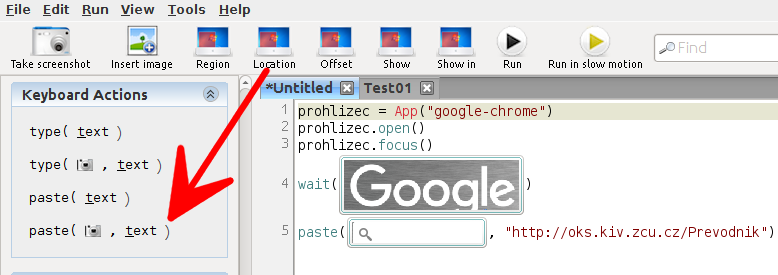
\includegraphics[width=12.5cm]{img/PrvniSkript/krok5.png}
					\end{figure}
					\FloatBarrier
				\item Na další řádku zadáme příkaz pro stisknutí klávesy Enter:\\\texttt{type(Key.ENTER)}
				\item V~prohlížeči otevřeme webovou stránku s~aplikací Převodník. V~SikuliX-IDE klikneme v~lévém menu na 
\includegraphics[scale=0.7]{img/PrvniSkript/click.png} a~provedeme screenshot záložky, která odkazuje na Převodník.
					\begin{figure}[ht!]
						\centering
						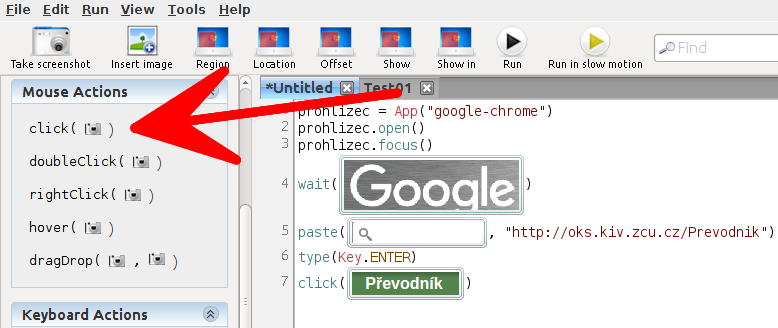
\includegraphics[width=12.5cm]{img/PrvniSkript/krok7.png}
					\end{figure}
					\FloatBarrier
				\item Klikneme na záložku aplikace Převodník. V~SikuliX-IDE opět vybereme 
\includegraphics[scale=0.7]{img/PrvniSkript/wait.png} a~uděláme snímek tlačítka \emph{Převeď}.
				\item Dále vybereme 
\includegraphics[scale=0.7]{img/PrvniSkript/paste.png} a~vytvoříme snímek vstupního pole. Snímek musí obsahovat popisek \emph{Vstup:}, aby byl jednoznačně identifikovatelný. Také musí obsahovat část vstupního pole dost velkou na to, aby ve středu snímku bylo toto pole, nikoli jeho okolí. Vložení hodnoty se provádí do středu snímku, což se ovšem dá upravit, jak si ukážeme v~dalším kroku. Jako druhý parametr zadáme hodnotu \texttt{"1"}.
				\item Vybereme možnost 
\includegraphics[scale=0.7]{img/PrvniSkript/click.png} a~vytvoříme screenshot obou výběrových seznamů. Nyní klikneme na obrázek seznamů v~SikuliX-IDE a~otevře se okno:
					\begin{figure}[ht!]
						\centering
						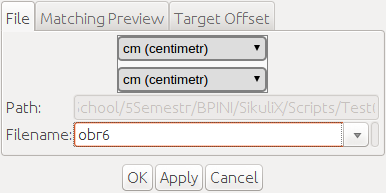
\includegraphics[width=10.5cm]{img/PrvniSkript/pattern.png}
					\end{figure}
					\FloatBarrier
					Klikneme na \emph{Target Offset}, které vypadá následovně:
						\begin{figure}[ht!]
						\centering
						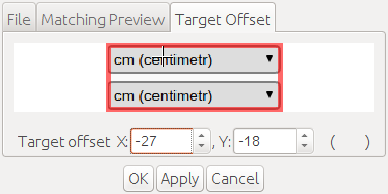
\includegraphics[width=10.5cm]{img/PrvniSkript/offset.png}
					\end{figure}
					\FloatBarrier
					Zde buď zadáme příslušné hodnoty do vstupních políček, nebo jen vybereme v~obrázku požadované místo. To nám zajistí, že SikuliX neklikne do středu obrázku, ale na zvolené místo v~něm. Potvrdíme tlačítkem \emph{OK} a~pokračujeme v~tvorbě skriptu.
				\item Nyní nastává problém. Potřebujeme vytvořit screenshot jedné položky ve výběrovém seznamu, ale SikuliX-IDE nám k tomu nedává možnost. Řešením je např. v~prohlížeči výběrový seznam rozbalit, provést screenshot celé obrazovky pomocí tlačítka \emph{PrintScreen} a~v~nějakém grafickém editoru vyříznout pouze tu část, kterou chceme (
\includegraphics[scale=0.8]{img/PrvniSkript/inch.png}). Tu poté uložíme do složky s~vytvářeným skriptem a~pouze doplníme následující kód: \texttt{click("nazev-snimku.png")}
				\item Na novou řádku napíšeme kód \texttt{click()} a~do závorek zkopírujeme výše použitý obrázek tlačítka \emph{Převeď}.
				\item Na další řádce si vytvoříme proměnnou \emph{vystup} a~přiřadíme do ní text z~výstupního textového pole. To se provede následujícím způsobem:\\\texttt{vystup = find("label-vystup.png").right(100).text()}\\
				Funkce \emph{right()} říká, že pracujeme s~oblastí širokou 100 pixelů napravo od nalezeného obrázku (popisku \emph{Výstup:}). Funkce \emph{text()} provede OCR\footnote{Optical Character Recognition -- optické rozpoznání znaků} a~vrátí zjištěný text.
					\begin{figure}[ht!]
						\centering
						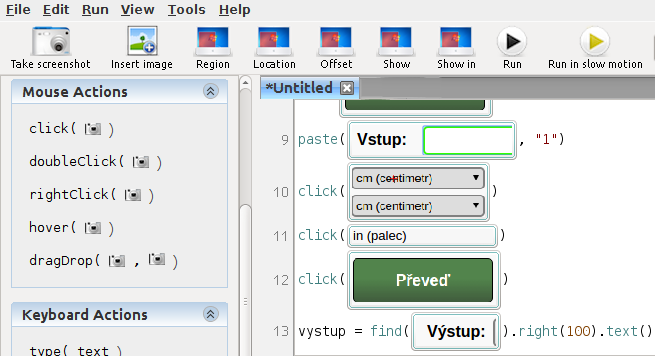
\includegraphics[width=12.5cm]{img/PrvniSkript/krok13.png}
					\end{figure}
					\FloatBarrier
				\item V~další části provedeme kontrolu zjištěného textu. Ten má obsahovat výslednou hodnotu -- 2.54. Vložíme do programu následující úsek kódu:\\\texttt{if vystup == "2.54":
					\\{\setlength{\parindent}{1cm}\indent popup("Ok textově")}
				\\else:
					\\{\setlength{\parindent}{1cm}\indent popError("Chyba")}}
				\item Další následuje \uv{optická} kontrola podle screenshotu. Potřebujeme si připravit do výstupního textového pole správný výsledek (hodnotu 2.54). To lze např. udělat tak, že provedeme převod hodnoty 2.54 mezi stejnými jednotkami. Jakmile se nám toto podaří, uděláme snímek výsledku a~uložíme jej ke skriptu. Zkopírujeme kód z~bodu 16. a~upravíme if-větev tak, že smažeme porovnání proměnné s~hodnotou a~napíšeme jako podmínku následující: \texttt{exists("nazev-snimku.png")}.
					\begin{figure}[ht!]
						\centering
						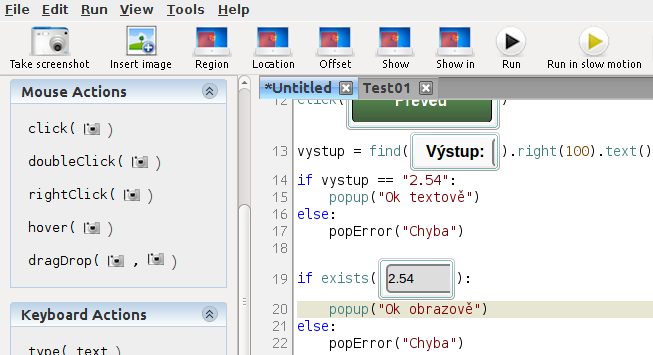
\includegraphics[width=12.5cm]{img/PrvniSkript/krok15.png}
					\end{figure}
					\FloatBarrier
				\item Jako poslední bod je zavření prohlížeče. To se provede příkazem\\\texttt{prohlizec.close()}.
			\end{enumerate}
			Tímto postupem by měl vzniknout skript téměř totožný s~tím, který je uveden v~kódu \ref{PrvniSkript}. Nebude obsahovat komentáře a~mohou se lišit názvy snímků.
		
			\begin{lstpython}{caption={První skript}, label={PrvniSkript}}
prohlizec = App("google-chrome")
prohlizec.open()	#otevre aplikaci definovanou
				#vyse
prohlizec.focus()	#vybere do popredi jeji okno
#ceka, dokud na obrazovce nenajde obrazek
wait("obr1.png")
#najde na obrazovce obrazek a vlozi do neho text
paste("obr2.png", "http://oks.kiv.zcu.cz/Prevodnik")
type(Key.ENTER)	#simuluje stisk klavesy ENTER
#najde na obrazovce obrazek a klikne na nej
click("obr3.png")
wait("obr4.png")
paste("obr5.png", "1")
#klikne o 27px vyse a 18px vlevo od nalezeneho
#obrazku
click(Pattern("obr6.png").targetOffset(-27,-18))
click("obr7.png")
click("obr4.png")
#precte text z casti, ktera je 100px vpravo od
#nalezeneho obrazku
vystup = find("obr8.png").right(100).text()
if vystup == "2.54":
	#pokud rozpoznany text souhlasi se zadanym,
	#otevre se vyskakovaci okno
    popup("Ok textove")
else:
    popError("Chyba")    #jinak se zobrazi chybove
    			 #okno

if exists("obr9.png"):
	#pokud na obrazovce existuje obrazek, otevre
	#se vyskakovaci okno
    popup("Ok obrazove")
else:
    popError("Chyba")
prohlizec.close()    #ukonci aplikaci
\end{lstpython}
		
	\section{Java API}
	Dále bylo zkoumáno Java API, které SikuliX poskytuje. Pro jeho použití je potřeba mít při překladu a~spuštění nastavený v~classpath \emph{sikulixapi.jar}. Toho docílíme např. tak, že použijeme v~příkazové řádce dvou příkazů\\\texttt{javac -cp sikulixapi.jar:. Test01.java}\\\texttt{java -cp sikulixapi.jar:. Test01}\\ Syntaxe, kterou SikuliX v~Java API využívá, je velmi podobná té v~SikuliX-IDE.
	
		\subsection{První test}
		První test s~použitím Java API, viz kód \ref{PrvniJavaAPI}, je téměř identický s~tím, který byl vytvořen pomocí SikuliX-IDE.
		
			\begin{lstjava}{caption={První test Java API}, label={PrvniJavaAPI}}
import org.sikuli.basics.Settings;
import org.sikuli.script.*;
import javax.swing.*;

public class Test01 {

  static Screen s;
  static App prohlizec;
  
  public static void main(String [] args) {
    Settings.OcrTextSearch = true;
    Settings.OcrTextRead = true;

    s= new Screen();
    prohlizec = new App("google-chrome");
    prohlizec.open();
    prohlizec.focus();
    
    try {
      s.wait("obr1.png");
      s.paste("obr2.png");
      s.type(Key.ENTER);
      s.click("obr3.png");
      s.wait("obr4.png");
      s.paste("obr5.png", "1");
      s.click(new Pattern("obr6.png").targetOffset(
        -27,-18));
      s.click("obr7.png");
      s.click("obr4.png");
      String t = s.find("obr8.png").right(
        100).text();
      if (Double.parseDouble(t) == 2.54) {
        JOptionPane.showMessageDialog(null, "Ok" +
          " textove");
      } else {
        JOptionPane.showMessageDialog(null, "Chyba");
      }
      if (s.exists("obr9.png") != null) {
        JOptionPane.showMessageDialog(null, "Ok" +
          " obrazove");
      } else {
        JOptionPane.showMessageDialog(null, "Chyba");
      }
      prohlizec.close();
    } catch (Exception e) {
      e.printStackTrace();
    }
  }
}
\end{lstjava}
	
		\subsection{Sofistikovanější testy}
		S~využitím knihoven \emph{JUnit} a~\emph{Log4j} (ani jedna z~těchto knihoven není pro běh SikuliX bezprostředně nutná) byly vytvořeny čtyři testy, viz kód \ref{DalsiJavaAPI}. První test skončí negativně, druhý pozitivně, třetí pozitivně a~čtvrtý negativně.
		
		Knihovna \emph{JUnit} byla použita z~toho důvodu, že nám pomůže jednak s~organizací testů a~jejich spouštěním, a~jednak s~jejich vyhodnocováním. Dále obsahuje metody pro vyhodnocování a~porovnávání hodnot, tzv. \emph{asserty}.
		
		\emph{Log4J} je knihovna, která slouží k~logování informací do souborů. Umožňuje vlastní konfiguraci výstupních souborů a~spoustu dalších funkcí. Použita byla z~toho důvodu, že během testování je vhodné zaznamenávat prováděné činnosti z důvodu jednoduššího zjištění případného selhání testu. SikuliX poskytuje informace o~tom, kam klikal či psal. Ty vypisuje na standardní výstup, avšak poskytuje metodu, které se předá instance \emph{Logger}, který poté SikuliX použije pro logování. Následuje ukázka zapisovaných informací, formátovaných vlastní konfigurací logeru, viz \ref{konfigurace}.
		{\lstset{basicstyle=\ttfamily\small}
		\begin{lstlisting}[]
18.04.2016 12:58:45 [INFO - TS03VymazaniJavaFX.
  invoke0()] - [info] runcmd: lsb_release -i -r -s
18.04.2016 12:58:46 [INFO - TS03VymazaniJavaFX.
  invoke0()] - [log] App.focus:  [1:PreVODNIK]
18.04.2016 12:58:50 [INFO - TS03VymazaniJavaFX.
  invoke0()] - [log] CLICK on L(925,298)@S(0)[0,0
  1920x1080]
18.04.2016 12:58:50 [INFO - TS03VymazaniJavaFX.
  invoke0()] - [log] CLICK on L(1128,298)@S(0)[0,0
  1920x1080]
18.04.2016 12:58:51 [INFO - TS03VymazaniJavaFX.
  invoke0()] - [log] CLICK on L(1128,422)@S(0)[0,0
  1920x1080]
18.04.2016 12:58:51 [INFO - TS03VymazaniJavaFX.
  invoke0()] - [log] CLICK on L(1128,333)@S(0)[0,0
  1920x1080]
18.04.2016 12:58:52 [INFO - TS03VymazaniJavaFX.
  invoke0()] - [log] CLICK on L(1127,457)@S(0)[0,0
  1920x1080]
18.04.2016 12:58:52 [INFO - TS03VymazaniJavaFX.
  invoke0()] - [log] CLICK on L(960,400)@S(0)[0,0
  1920x1080]
18.04.2016 12:58:53 [INFO - TS03VymazaniJavaFX.
  invoke0()] - [log] CLICK on L(960,587)@S(0)[0,0
  1920x1080]
18.04.2016 12:58:58 [ERROR - TS03VymazaniJavaFX.
  TC03_01_02PrevodChyba()] - Vstupni vyberovy seznam
  nema defaultni hodnotu
18.04.2016 12:58:59 [INFO - TS03VymazaniJavaFX.
  invoke0()] - [log] CLICK on L(661,198)@S(0)[0,0
  1920x1080]
	\end{lstlisting}}